\documentclass[a4paper,11pt]{report}
\usepackage[german, english]{babel} % Languages
\usepackage{tikz} % Tikz figures
\usepackage{siunitx} % SI-units package
\usepackage{bm} % Bold mathematics
\usepackage{listings} % Make listings, e.g. for code
\usepackage{enumitem} % Enumerate and itemize commands
\usepackage{multicol} % Make multiple columns for content
\usepackage[left=15mm, right=15mm, bottom=15mm, top=15mm, includeheadfoot]{geometry} % Modify geometry of page format
\usepackage{placeins} % For float barrier command
\usepackage{amsmath} % Math environments
\usepackage{fancyhdr} % Include the fancyhdr package
\usepackage{amsthm} % Theorem environments
\usepackage{siunitx} % Use SI
\usepackage{array} % Use array package for tables
\usepackage{tabularx} % Package to make nice tables
\usepackage{amssymb} % Math symbols
\usepackage{lipsum} % Provide dummy text
\usepackage{abstract} % Abstract package
\usepackage{nicefrac} % Nice fractions in in-line texts
\usepackage[hidelinks]{hyperref} % Make document with hyperlinks
\usepackage{cleveref} % Make references
\usepackage{subcaption} % Make subfigures
\usepackage{graphicx} % Make figures
\usepackage{mhchem} % Chemical notation
\usepackage{mathtools} % Various math tools
\usepackage{framed} % Frame equations
% Figure caption setup
\captionsetup{font=footnotesize,labelfont=bf}

% Python code listings
\definecolor{codegreen}{rgb}{0,0.6,0}
\definecolor{codegray}{rgb}{0.5,0.5,0.5}
\definecolor{codepurple}{rgb}{0.58,0,0.82}
\definecolor{backcolour}{rgb}{0.95,0.95,0.92}

\lstdefinestyle{mystyle}{
	backgroundcolor=\color{backcolour},   
	commentstyle=\color{codegreen},
	keywordstyle=\color{magenta},
	numberstyle=\tiny\color{codegray},
	stringstyle=\color{codepurple},
	basicstyle=\ttfamily\footnotesize,
	breakatwhitespace=false,         
	breaklines=true,                 
	captionpos=b,                    
	keepspaces=true,                 
	numbers=left,                    
	numbersep=5pt,                  
	showspaces=false,                
	showstringspaces=false,
	showtabs=false,                  
	tabsize=2
}

% Enumerate style
\renewcommand{\theenumi}{(\arabic{enumi})}
\renewcommand\labelenumi{\theenumi} % Change enumerate style from 1. to (1) etc.
\renewcommand{\theenumiii}{(\arabic{enumiii})}
\renewcommand\labelenumiii{\theenumiii} % Change enumerate style from 1. to (1) etc.
\setlist{itemsep = 0.2pt}

% Matrix and vector notation
\newcommand\matr[1]{\ensuremath{\boldsymbol{\mathbf{#1}}}}
\newcommand\vect[1]{\ensuremath{\bm{#1}}}
\newcommand\dint{\ensuremath{\int\displaylimits}}

% Units definitions
\DeclareSIUnit \parsec {pc}
\DeclareSIUnit \magnitudes {mag}

% Theorem environment
\newtheorem{tm}{Theorem}
\numberwithin{tm}{subsection}

% New tag form
\newtagform{normalsize}[\normalsize]{\normalsize(}{\normalsize)}

% Configure head- and footlines
\pagestyle{fancy} % Set head- and footlines
\fancyhead[C]{Adult face predicting machine} % Left headline
\fancyhead[L]{\nouppercase{\leftmark}} % Right headline
\fancyhead[R]{D. Zahnd, R. Zahnd}

\author{Daniel Zahnd}
\date{May 11, 2023 - \today}
\title{Water rocket physics \\ \vspace{0.5cm} \normalsize An analysis of the physical principles of a water rocket}

%, including a building plan and launching recommendations

\begin{document}
\begin{titlepage}
    %\newgeometry{margin=2in} % Adjust margins for the title page
    
    \centering
    
    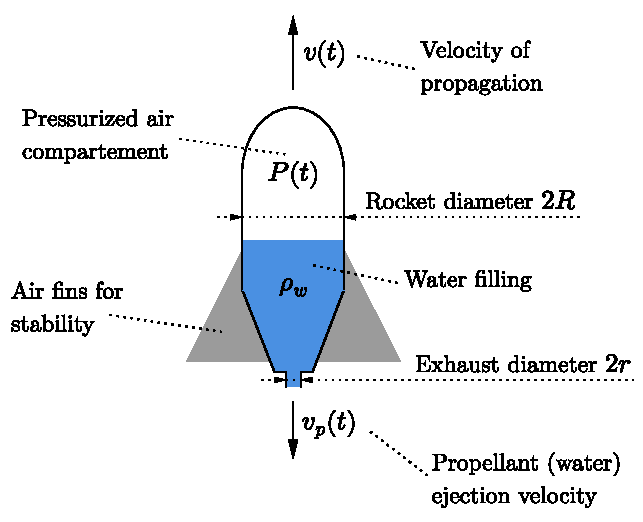
\includegraphics[width=\textwidth-3cm]{figures/setupcalculations.pdf} % Replace 'your_image.jpg' with the actual image file name and path
    
    \vspace{2cm}
    
    \Huge
    \textbf{Water Rocket Physics}
    
    \vspace{0.5cm}
    
    \normalsize
    An analysis of the physical principles of a water rocket
    
    \vspace{3cm}
    
    \Large
    \text{Daniel Zahnd}
    
    \vfill
    
    \large
    May 11, 2023 - \today % Date will automatically update
    
    %\restoregeometry % Restore default margins for the rest of the document
\end{titlepage}

%\begin{document}
%\usetagform{normalsize}
%\maketitle
%\tableofcontents

%\newgeometry{left=40mm,right=40mm}

\newpage
\pagenumbering{roman}
\tableofcontents
\FloatBarrier
\newpage
\pagenumbering{arabic}
\setcounter{page}{1}

\chapter{Introduction}
The principle upon which rockets rely is simply Newton's third law, also known as the \textit{actio est reactio} principle. Newton's third law states, that whenever there are two entities $A$ and $B$ and $A$ exerting a force $\vect{F}_{A\rightarrow B}$ upon $B$, there is also a force $\vect{F}_{B\rightarrow A}$ which is exerted on $A$ by $B$ related to $\vect{F}_{A\rightarrow B}$ as \begin{equation}
\vect{F}_{A\rightarrow B} = -\vect{F}_{B\rightarrow A}.
\end{equation} A rocket in general is therefore a prime example of Newton's third law, but also of the conservation of momentum, meaning that all momenta $\vect{p}_i(t),\,i\in\{1,\dots,n\},\,n\in\mathbb{N}$ in the system `` rocket'' add up to zero at all times $t$, that is 
$\sum_i \vect{p}_i(t) = 0$. Using the second law of Newton, the momenta $\vect{p}_i(t)$ in the system can be connected to forces $\vect{F}_i(t)$ as \begin{equation}
\vect{F}_i(t) = \frac{\mathrm{d}}{\mathrm{d}t}\vect{p}_i(t),
\end{equation} which allows for a derivation of the equation of motion for a rocket.

One of the first people to find and publish a form of the so-called rocket equation, namely Russian rocket scientist Konstantin Tsiolkovsky, proposed the following thought experiment. Imagine sitting on a rowing boat loaded with several individual stones; by an unhappy accident, you loose your oars, giving rise to the problem that your boat is no longer maneuverable. Remembering the physics education you received in school, you immediately have an idea to solve this problem looking at the stones loaded in your boat. By throwing the stones into the water in opposite direction of where you want to go one after another, you can propel the boat safely to shore. This is because by throwing a stone into the water, you exert a force $\vect{F}_{\text{boat}\rightarrow \text{water}}$ on the boat, but due to Newton's third law, an opposite force $\vect{F}_{\text{water}\rightarrow \text{boat}} = -\vect{F}_{\text{boat}\rightarrow \text{water}}$ is exerted by the water on the boat, propelling it to shore. In this case, the stones served as a propellant, but with a water rocket, also water can be used as a propellant - in fact, any massive substance can be used as a propellant for a rocket or other vehicles; the only condition for a propellant is, that it is ejected from the vehicle with high velocity, generating thrust to move the vehicle forward.

Using water as a propellant - rather than hot gases ejected from a jet engine - these Newtonian principles can be turned into action by means of building a water rocket.

\chapter{Setup}
A water rocket is essentially a container partially filled by water, where the remaining space contains pressurized air. The water rocket consists of a single opening at the bottom, through which the water contained in the rocket is ejected due to pressure chamber in the rocket, which is pressurized by several atmospheres, creating quite a significant pressure gradient with respect to the environment.

The water rocket is filled to approximately one third by water and by two thirds with pressurized air; the pressurization can be undertaken by means of a bicycle pump. Using a suitable release mechanism, the rocket can be allowed to depressurize, resulting in the ejection of the water from the rocket and therefore producing thrust for the rocket; thrust is generated - as briefly explained in the introduction - by application of Newton's second and third laws of mechanics. A sketch of the setup may be found in \cref{fig:setup}.
\begin{figure}[h!]
\centering
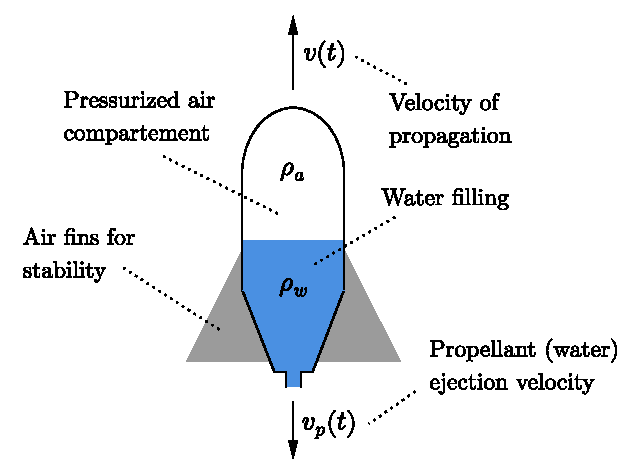
\includegraphics[height=6cm]{figures/setup.pdf}
\caption{Sketch of a water rocket. Such a water rocket can be built using simple tools and resources; a water bottle, some styrofoam for the fins, hot glue and some hosing tools and equipment.}
\label{fig:setup}
\end{figure}

\chapter{Analysis}
\section{Physics and mathematics preliminaries}
\subsection{Bernoulli equation}
The Bernoulli equation relates the pressure $P(\vect{x},t)$ of a fluid element along a streamline with the respective velocity $\vect{v}(\vect{x},t)$ and height $h(\vect{x},t)$ above ground of the fluid element. The change of any quantity along a streamline is given by the operator $\vect{v}(\vect{x},t)\cdot \vect{\nabla}$, which is a derivative parallel to $\vect{v}(\vect{x},t)$. The Bernoulli equation states, that \begin{equation}
P(\vect{x},t) + \rho g h(\vect{x},t) + \frac{1}{2}\rho \vect{v}(\vect{x},t)^2 = \text{const.}
\end{equation} holds. Consider all quantities at a fixed time $t$ and at two places $\vect{x}_1$ and $\vect{x}_2$ along a streamline; let $P(\vect{x}_1,t) \doteq P_1$, $P(\vect{x}_2,t) \doteq P_2$, $h(\vect{x}_1,t) \doteq h_1$, $h(\vect{x}_2,t) \doteq h_2$, $\vect{v}(\vect{x}_1,t) \doteq \vect{v}_1$ and $\vect{v}(\vect{x}_2,t) \doteq \vect{v}_2$; then, the Bernoulli equation can also be stated in the form
\begin{equation}
P_1 + \rho h_1 g + \frac{1}{2}\rho \vect{v}_1^2 = P_2 + \rho h_2 g + \frac{1}{2}\rho \vect{v}_2^2,
\end{equation} where $g \approx \SI{9.81}{\meter\second^{-2}}$ is the gravitational acceleration. The Bernoulli equation in these formulations only holds for incompressible fluids, which is to say that the density $\rho$ across the fluid essentially stays the same everywhere in the system under consideration at all times.

\subsection{Drag equation}
The so-called drag equation relates the velocity $\vect{v}(t)$ of an object to the force $\vect{F}_d(t)$ exerted on it by friction between the object and the surrounding medium. The drag equation is given by \begin{equation}
\vect{F}_d(\vect{x},t) = -\frac{1}{2}\rho(\vect{x}) C_d A\frac{\vect{v}(t)^3}{|\vect{v}(t)|}, 
\end{equation} where $\rho(\vect{x})$ is the density of the surrounding medium, $C_d$ is the so-called drag coefficient of the object travelling with speed $\vect{v}(t)$ and $A$ is the cross-sectional area of the object with respect to its propagation direction. By definition, the drag force is directed exactly opposed to the propagation direction of the object at all times $t$.

The drag coefficient $C_d$ is dependent upon the geometry of the object. Different coefficients can be taken from \cref{fig:dragcoefficients}.
\begin{figure}[h!]
\centering
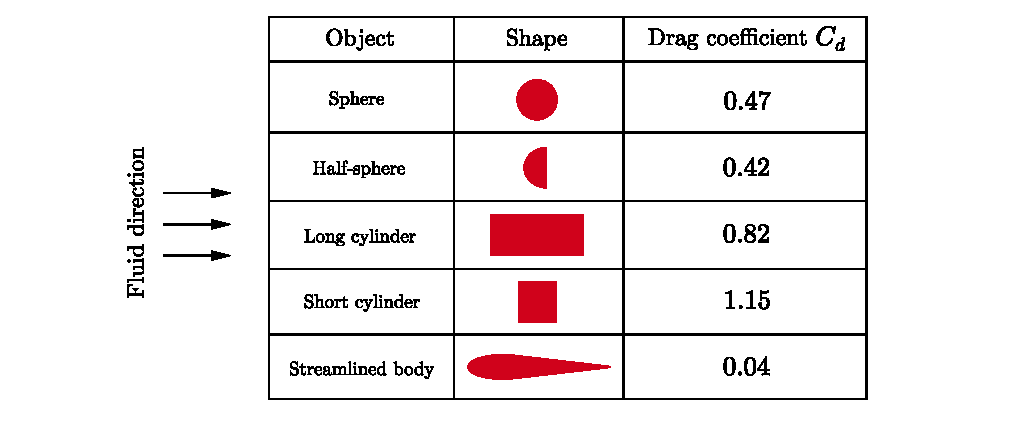
\includegraphics[width=11cm]{figures/dragcoefficients.pdf}
\caption{Drag coefficients for different object geometries.}
\label{fig:dragcoefficients}
\end{figure} A water rocket made from a plastic bottle combines the properties of a sphere, of a half-sphere aswell as of a long cylinder; therefore it seems reasonable to calculate an average drag coefficient $\bar{C_{d}}$ for the water rocket averaging over these three shapes, given by \begin{equation}\label{eq:avdragvalue}
\bar{C_{d}} = \frac{C_{d,s}+C_{d,hs}+C_{d,lc}}{3} = 0.57.
\end{equation}

\subsection{Rocket equation}
Consider a rocket ascending in positive vertical direction, where the speed of the rocket is denoted by $\vect{v}(t)$ and the propellant is ejected with velocity $\vect{v}_p(t)$ in negative vertical direction. The rocket equation can be stated as \begin{equation}
m(t)\frac{\mathrm{d}\vect{v}(t)}{\mathrm{d}t} = \frac{\mathrm{d}m(t)}{\mathrm{d}t}\vect{v}_p(t)\theta(\tau-t) - \frac{1}{2}\rho(\vect{x})\vect{v}(t)^2\bar{C}_dA\vect{e}_z - m(t)g\vect{e}_z, 
\end{equation} where $\tau$ denotes the total time of propellant ejection. Given the stated assumptions and furthermore assuming a constant surrounding density $\rho$ for all places $\vect{x}$ and times $t$, the rocket velocity is $\vect{v}(t) = |\vect{v}(t)|\vect{e}_z = v(t)\vect{e}_z$ and the propellant velocity can be written as $\vect{v}_p(t) = -|\vect{v}_p(t)|\vect{e}_z = -v_p(t)\vect{e}_z$, simplifying the rocket equation to \begin{equation}\label{eq:rocketeqsimple}
m(t)\frac{\mathrm{d}v(t)}{\mathrm{d}t} = -\frac{\mathrm{d}m(t)}{\mathrm{d}t}v_p(t)\theta(\tau-t) - \frac{1}{2}\rho \bar{C}_d A v(t)^2 - m(t) g.
\end{equation} Here, the so-called Heaviside function
\begin{equation}\label{eq:defheaviside}
\theta: \mathbb{R} \rightarrow \{0,1\}, \quad t \mapsto \theta(t) = \begin{cases}
1, & t > 0 \\
0, & t \leq 0
\end{cases}
\end{equation} was used.

\subsection{Integrals using the Heaviside function}
Consider the above defined Heaviside function \cref{eq:defheaviside} and three functions defined as \begin{equation}
g(t)\doteq f(t)\theta(\tau-t), \quad h(t) \doteq f(t)\theta(t-\tau), \quad k(t) \doteq f(\tau)\theta(t-\tau),
\end{equation} where $f(t)$ is an arbitrary smooth function. The integral of $g(t)$ with respect to time $t$ can be calculated as \begin{align}\label{eq:heavisideintegrate_1}
\begin{aligned}
I_{g(t)} &= \int_{0}^{t}g(t^\prime)\,\mathrm{d}t^\prime = \int_{0}^{t} f(t^\prime)\theta(\tau-t^\prime)\,\mathrm{d}t^\prime \\
&= \theta(t-\tau)\int_{0}^{\tau}f(t^\prime)\,\mathrm{d}t^\prime + \theta(\tau-t)\int_{0}^{t}f(t^\prime)\,\mathrm{d}t^\prime.
\end{aligned}
\end{align} The integral of $h(t)$ with respect to time $t$ can be calculated as \begin{align}\label{eq:heavisideintegrate_2}
\begin{aligned}
I_{h(t)} &= \int_{0}^{t}h(t^\prime)\,\mathrm{d}t^\prime = \int_{0}^{t} f(t^\prime)\theta(t^\prime-\tau)\,\mathrm{d}t^\prime \\
&= \theta(t-\tau)\int_{\tau}^{t}f(t^\prime)\,\mathrm{d}t^\prime + \theta(\tau-t)\cdot 0 \\
&= \theta(t-\tau)\int_{\tau}^{t}f(t^\prime)\,\mathrm{d}t^\prime.
\end{aligned}
\end{align} The integral of $k(t)$ with respect to time $t$ can be calculated as \begin{align}\label{eq:heavisideintegrate_3}
\begin{aligned}
I_{k(t)} &= \int_{0}^{t}k(t^\prime)\,\mathrm{d}t^\prime = \int_{0}^{t} f(\tau)\theta(t^\prime-\tau)\,\mathrm{d}t^\prime \\
&= \theta(t-\tau)f(\tau)\int_{\tau}^{t}\,\mathrm{d}t^\prime + \theta(\tau-t)f(\tau)\cdot 0 \\
&= \theta(t-\tau)f(\tau)\int_{\tau}^{t}\,\mathrm{d}t^\prime.
\end{aligned}
\end{align}

\section{Solving the rocket equation for a water rocket not experiencing drag force}
Solving the rocket equation without taking drag forces into consideration can be done analytically. In this section, the analytical solution for the rocket equation without drag force is derived, as well as examined by example calculations.

\subsection{Formulation of the rocket equation for a water rocket not experiencing drag force}
In order to solve the rocket equation without taking into consideration drag forces exerted by the air surrounding the rocket, we start from \cref{eq:rocketeqsimple}. Not accounting for drag forces means, that the drag coefficient $\bar{C}_d$ is set to zero, that is $\bar{C}_d = 0$. Therefore, the second term in \cref{eq:rocketeqsimple} vanishes and we can account for the resulting rocket equation by \begin{equation}
m(t)\frac{\mathrm{d}v(t)}{\mathrm{d}t} = -\frac{\mathrm{d}m(t)}{\mathrm{d}t}v_p(t)\theta(\tau-t) - m(t) g,
\end{equation} where $v_p(t) \geq 0$. Furthermore, we assume, that the propellant velocity is constant, i.e. $v_p(t) = v_p$, whereas for the mass of the rocket, a linear relationship to time is presupposed. Hence, the mass $m(t)$ can be accounted for by \begin{equation}
m(t) = m_0 - bt \quad \Rightarrow \quad \frac{\mathrm{d}m(t)}{\mathrm{d}t} = -b,
\end{equation} with $b$ being the mass ejection parameter with units $[b] = \si{\kilo\gram\second^{-1}}$. Using these simplifications, the rocket equation can be further simplified to \begin{equation}
(m_0-bt)\frac{\mathrm{d}v(t)}{\mathrm{d}t} = bv_p\theta(\tau-t) - (m_0-bt) g.
\end{equation} Dividing both sides of this equation by $m_0-bt$ yields \begin{equation}\label{eq:rocketeqwithoutdragtointegrate}
\frac{\mathrm{d}v(t)}{\mathrm{d}t} = \frac{bv_p}{m_0-bt}\theta(\tau-t)-g,
\end{equation} which can subsequently be integrated with respect to time $t$.

\subsection{Analytical solution of the rocket equation for a rocket not experiencing drag force}
In order to obtain the velocity $v(t)$ of the rocket, \cref{eq:rocketeqwithoutdragtointegrate} has to be integrated with respect to time $t$, that is to say by calculating \begin{equation}
v(t) = \int_{0}^{t} \frac{\mathrm{d}v(t^\prime)}{\mathrm{d}t^\prime}\,\mathrm{d}t^\prime = \int_{0}^{t} \left[\frac{bv_p}{m_0-bt^\prime}\theta(\tau-t^\prime)-g\right]\,\mathrm{d}t^\prime.
\end{equation} The integral on the right-hand side of the above equation can be split into three parts by application of \cref{eq:heavisideintegrate_1}, such that \begin{gather}\small\begin{gathered}
v(t) \overset{\text{\cref{eq:heavisideintegrate_1}}}{=} \underbrace{\theta(t-\tau)\int_{0}^{\tau} \frac{bv_p}{m_0-bt^\prime}\,\mathrm{d}t^\prime}_{I_{v,1}} + \underbrace{\theta(\tau-t)\int_{0}^{t}\frac{bv_p}{m_0-bt^\prime}\,\mathrm{d}t^\prime}_{I_{v,2}} - \underbrace{\int_{0}^{t}g\,\mathrm{d}t^\prime}_{I_{v,3}}.
\end{gathered}\end{gather} Solving the integrals $I_{v,1}$ and $I_{v,2}$ can be solved by means of using the integral \begin{equation}
\int_{0}^{t}\frac{bv_p}{m_0-bt^\prime}\,\mathrm{d}t^\prime = -v_p\int_{m_0}^{m_0-bt} \frac{1}{x}\,\mathrm{d}x = v_p \ln\left(\frac{m_0}{m_0-bt}\right),
\end{equation} where the substitution $x(t^\prime) \doteq m_0-bt^\prime$ was performed; hence for $I_{v,1}$, $I_{v,2}$ and $I_{v,3}$ one obtains 
$I_{v,1} = \theta(t-\tau)v_p\ln\left(\frac{m_0}{m_0-b\tau}\right)$, $I_{v,2} = \theta(\tau-t)v_p\ln\left(\frac{m_0}{m_0-bt}\right)$ and $I_{v,3} = gt$. Putting everything together yields \begin{equation}\label{eq:rocketvelocitywithoutdrag}
v(t) = \theta(t-\tau)v_p\ln\left(\frac{m_0}{m_0-b\tau}\right) + \theta(\tau-t)v_p\ln\left(\frac{m_0}{m_0-bt}\right) - gt.
\end{equation}

In order to obtain the analytical expression for the height $h(t)$ reached by the rocket, \cref{eq:rocketvelocitywithoutdrag} has to be integrated with respect to time $t$, that is to say by calculating
\begin{equation}
h(t) = \int_{0}^{t} \frac{\mathrm{d}h(t^\prime)}{\mathrm{d}t^\prime}\,\mathrm{d}t^\prime = \int_{0}^{t}v(t^\prime)\,\mathrm{d}t.
\end{equation} Using the expression \cref{eq:rocketvelocitywithoutdrag}, one obtains \begin{align}\begin{aligned}
h(t) &= \underbrace{\int_{0}^{t}\theta(t^\prime-\tau)v_p\ln\left(\frac{m_0}{m_0-b\tau}\right)\,\mathrm{d}t^\prime}_{I_{h,1}} \\  &+ \underbrace{\int_{0}^{t}\theta(\tau-t^\prime)v_p\ln\left(\frac{m_0}{m_0-bt^\prime}\right)\,\mathrm{d}t^\prime}_{I_{h,2}} - \underbrace{\int_{0}^{t}gt^\prime\,\mathrm{d}t^\prime}_{I_{h,3}}.
\end{aligned}\end{align} The integral $I_{h,1}$ can be solved by using \cref{eq:heavisideintegrate_3}, such that \begin{align}\begin{aligned}
I_{h,1} &= \int_{0}^{t}\theta(t^\prime-\tau)v_p\ln\left(\frac{m_0}{m_0-b\tau}\right)\,\mathrm{d}t^\prime \\ &\overset{\text{\cref{eq:heavisideintegrate_3}}}{=} \theta(t-\tau)v_p\ln\left(\frac{m_0}{m_0-b\tau}\right)\int_{\tau}^{t}\,\mathrm{d}t^\prime \\
&= \theta(t-\tau)v_p\ln\left(\frac{m_0}{m_0-b\tau}\right)(t-\tau).
\end{aligned}\end{align} The integral $I_{h,2}$ is more complicated to solve; first, it can be decomposed into two separate parts using \cref{eq:heavisideintegrate_1}, yielding \begin{align}\begin{aligned}
I_{h,2} &\overset{\text{\cref{eq:heavisideintegrate_1}}}{=} \underbrace{\theta(t-\tau)v_p\int_{0}^{\tau}\ln\left(\frac{m_0}{m_0-bt^\prime}\right)\,\mathrm{d}t^\prime}_{I_{h,2a}} \\ &\qquad \, + \underbrace{\theta(\tau-t)v_p\int_{0}^{t}\ln\left(\frac{m_0}{m_0-bt^\prime}\right)\,\mathrm{d}t^\prime}_{I_{h,2b}}.
\end{aligned}\end{align} Solving these integrals requires the solution to an integral of the form \begin{align}\label{eq:solvehintegrals}
\begin{aligned}
\int_{0}^{t} \ln\left(\frac{m_0}{m_0-bt^\prime}\right)\,\mathrm{d}t^\prime &= \frac{m_0}{b}\int_{1}^{\tfrac{m_0}{m_0-bt}}\frac{\ln(y)}{y^2}\,\mathrm{d}y \\ &= -\frac{m_0}{b}\int_{1}^{\tfrac{m_0}{m_0-bt}}\frac{\mathrm{d}}{\mathrm{d}y}\left(\frac{\ln(y)+1}{y}\right)\,\mathrm{d}y \\
%&= -\frac{m_0}{b}\left[\frac{\ln(y)+1}{y}\right]_1^{\tfrac{m_0}{m_0-bt}} \\ &= -\frac{m_0}{b}\left[\frac{m_0-bt}{m_0}\ln\left(\frac{m_0}{m_0-bt}\right) + \frac{m_0-bt}{m_0}-1\right] \\ 
&= t- \frac{m_0-bt}{b}\ln\left(\frac{m_0}{m_0-bt}\right),
\end{aligned}
\end{align} where the substitution $y(t^\prime) \doteq \tfrac{m_0}{m_0-bt^\prime}$ was used. Using this integral, one obtains \begin{equation}
I_{h,2a} = \theta(t-\tau)v_p\left[\tau- \frac{m_0-b\tau}{b}\ln\left(\frac{m_0}{m_0-b\tau}\right)\right]
\end{equation} and \begin{equation}
I_{h,2b} = \theta(\tau - t)v_p\left[t- \frac{m_0-bt}{b}\ln\left(\frac{m_0}{m_0-bt}\right)\right],
\end{equation} herewith obtaining $I_{h,2}$ as \begin{align}\begin{aligned}
I_{h,2} &= \theta(t-\tau)v_p\left[\tau- \frac{m_0-b\tau}{b}\ln\left(\frac{m_0}{m_0-b\tau}\right)\right] \\ &\quad + \theta(\tau - t)v_p\left[t- \frac{m_0-bt}{b}\ln\left(\frac{m_0}{m_0-bt}\right)\right].
\end{aligned}\end{align} Hence, the total solution to $h(t)$ is yielded by the expression $h(t) = I_{h,1} + I_{h,2} - I_{h,3}$, given by \begin{align}\label{eq:generalanalyticalsolution}
\small\begin{aligned}
h(t) &= \theta(t-\tau)v_p\left[\ln\left(\frac{m_0}{m_0-b\tau}\right)(t-\tau) + \tau-\frac{m_0-b\tau}{b}\ln\left(\frac{m_0}{m_0-b\tau}\right)\right] \\
&\quad + \theta(\tau-t)v_p\left[t-\frac{m_0-bt}{b}\ln\left(\frac{m_0}{m_0-bt}\right)\right] - \frac{1}{2}gt^2.
\end{aligned}
\end{align}

\subsection{Propellant velocity, propellant ejection time and mass ejection parameter}
In order to calculate the propellant velocity $v_p$, the propellant ejection time $\tau$ and the mass ejection parameter $b$ needed to perform actual calculations using the solutions of the rocket equation, the Bernoulli equation can be of help; consider therefore \cref{fig:setupcalculations}.
\begin{figure}[h!]
\centering
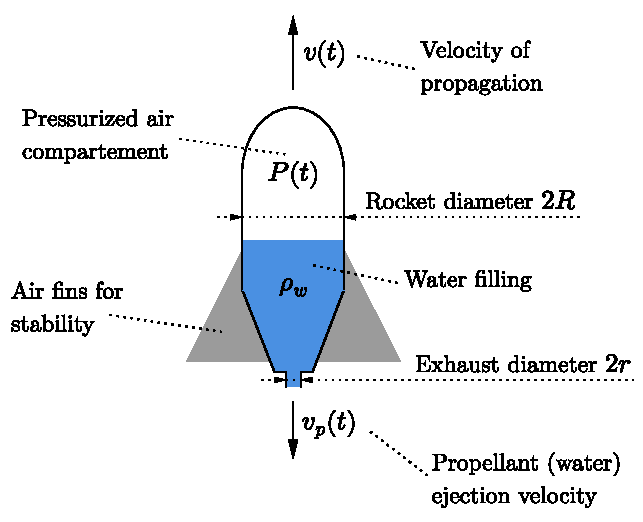
\includegraphics[height=6cm]{figures/setupcalculations.pdf}
\caption{Sketch of a water rocket with necessary definitions of quantities to calculate.}
\label{fig:setupcalculations}
\end{figure}

In order to use the Bernoulli equation to calculate an approximate expression for the propellant velocity $v_p(t) = v_p$ - which is assumed to be constant over the whole period of propellant ejection -, one first needs to know the function $P(t)$. The function $P(t)$ describes, how the pressure inside the pressurized air chamber of the rocket evolves in time, as the water is ejected through the exhaust. In order to keep things as simple as possible, but still powerful regarding predictions, a linear relationship $P(t) = \alpha_P t + P_0$ for the pressure is assumed, where we require, that $P(\tau) = 0$ and $P(0) = P_0$. This means, that the slope parameter $\alpha_P$ must be given as $\alpha_P = -P_0/\tau$. The pressure $P(t)$ is understood to be the additional pressure to one standard atmosphere, which is to say that it is the pressure indicated by any pump or pressure measuring device. If the propellant ejection velocity $v_p$ is assumed to be constant, it is reasonable to use averaged values with respect to time in calculations leading to an expression for $v_p$. The, we calculate the average pressure $\bar{P}$ over the total time of propellant ejection as \begin{align}\small\begin{aligned}
\bar{P} = \frac{1}{\tau}\int_{0}^{\tau} P(t)\,\mathrm{d}t = \frac{1}{\tau}\int_{0}^{\tau} [\alpha_P t + P_0]\,\mathrm{d}t = \frac{1}{2}\alpha_P\tau + P_0 = -\frac{P_0}{2} + P_0 = \frac{P_0}{2}.
\end{aligned}\end{align} For coarse approximation purposes is reasonable to use average values for any time dependent quantity, hence we use $P(t) \approx \bar{P}$.

Next, we assume, that the flow velocity of the fluid inside the rocket is zero; furthermore, any gravitational effect within the fluid is neglected. It is to be remembered, that $P(t) \approx \bar{P}$ describes the pressure that exceeds that of one standard atmosphere. Using the Bernoulli equation, one therefore obtains the equation \begin{equation}\label{eq:propellantejectionvelocity}
\bar{P} = \frac{1}{2}\rho_w v_p^2 \quad \Leftrightarrow \quad v_p = \sqrt{\frac{2\bar{P}}{\rho_w}} = \sqrt{\frac{P_0}{\rho_w}}.
\end{equation}

The propellant ejection time $\tau$ is calculated using the assumption, that the total mass of water $m_{w}$ initially present in the rocket tank is equal to a cylinder of water with a height $v_p\tau$ and a radius of $r$; $r$ being the exhaust radius. Denoting the mass of the empty rocket with $m_r$, it hence follows, that \begin{equation}\label{eq:propellantejectiontime}
m_{w} = m_0 - m_r = \rho_wr^2\pi v_p\tau = r^2 \pi \tau \sqrt{P_0\rho_w} \quad \Leftrightarrow \quad \tau = \frac{m_w}{r^2\pi \sqrt{P_0 \rho_w}}
\end{equation} holds.

Now, it is straightforward to calculate the mass ejection parameter $b$ involved in the mass equation $m(t) = m_0 - bt = m_w + m_r - bt;$ for this purpose, we require $m(\tau) = m_r$. Hence, the parameter $b$ is the obtained as \begin{equation}\label{eq:freeparameters}
m(\tau) = m_w + m_r -b\tau = m_r \quad \Leftrightarrow \quad b = \frac{m_w}{\tau} = r^2\pi \sqrt{P_0\rho_w}.
\end{equation}

\subsection{Maximal height}
Given that the typical timespan \begin{equation}
\tau = \frac{m_w}{r^2\pi \sqrt{P_0 \rho_w}}
\end{equation} of water ejection is very short compare to the total flight time of a water rocket, we can restrict the time interval where we look for maximal height to the condition $t > \tau$, since the rocket is very likely to be in upward vertical motion while propellant is still ejected. Due to inertia, the rocket will even be in upward motion for a time period after the last bit of propellant was ejected, hence the restriction $t > \tau$ in time for a search of maximal height optimization. With this restriction, the general solution \cref{eq:generalanalyticalsolution} now just reads as \begin{gather}\small\begin{gathered}
h(t) = v_p \left[\ln\left(\frac{m_0}{m_0-b\tau}\right)(t-\tau)+\tau - \frac{m_0-b\tau}{b}\ln\left(\frac{m_0}{m_0-b\tau}\right)\right] - \frac{1}{2}gt^2.
\end{gathered}\end{gather} Basically, there are two controllable parameters with a water rocket, the mass of the water $m_w$ with which the rocket was filled; and the pressure $P_0$ the rocket is started with. For further optimization, we first need to find an expression for maximal height $h_{max}(m_w,P_0)$ involving these parameters, so we start by the classical procedure for finding an extremal point of a function:
\begin{align}
\frac{\mathrm{d}h(t)}{\mathrm{d}t} = v_p \ln\left(\frac{m_0}{m_0-b\tau}\right) - gt \overset{!}{=} 0,
\end{align} which leads to the time of maximal height $t_{max}$ as \begin{equation}
t_{max} = \frac{v_p}{g}\ln\left(\frac{m_0}{m_0-b\tau}\right)
\end{equation} by means of rearrangement. Now, we can calculate $h_{max}$ by just inserting $t_{max}$ into the function $h(t)$ for $t$:
\begin{align}\begin{aligned}
h(t_{max}) &= v_p\ln\left(\frac{m_0}{m_0-b\tau}\right)\frac{v_p}{g}\ln\left(\frac{m_0}{m_0-b\tau}\right)-v_p\ln\left(\frac{m_0}{m_0-b\tau}\right)\tau \\ &\quad + v_p\tau - \frac{m_0-b\tau}{b}v_p\ln\left(\frac{m_0}{m_0-b\tau}\right) \\
%&= v_p\ln\left(\frac{m_0}{m_0-b\tau}\right)\left[\frac{v_p}{g}\ln\left(\frac{m_0}{m_0-b\tau}\right)-\tau-\frac{m_0}{b}+\tau\right] + v_p\tau \\
&= v_p\ln\left(\frac{m_0}{m_0-b\tau}\right)\left[\frac{v_p}{g}\ln\left(\frac{m_0}{m_0-b\tau}\right)-\frac{m_0}{b}\right] + v_p\tau.
\end{aligned}\end{align} Inserting the full expressions for the parameters $b$ and $\tau$ as given in \cref{eq:freeparameters} finally yields a function \begin{align}\footnotesize\begin{aligned}
h_{max}(m_w,P_0) &= \sqrt{\frac{P_0}{\rho_w}}\ln\left(\frac{m_f+m_w}{m_f}\right)\left[\sqrt{\frac{P_0}{g^2\rho_w}}\ln\left(\frac{m_f + m_w}{m_f}\right)-\frac{m_f + m_w}{r^2\pi \sqrt{P_0\rho_w}}\right]  \\ &\quad + \frac{m_w}{r^2\pi\rho_w}.
\end{aligned}\end{align} By using multidimensional calculus, one could now in principle optimize $h_{max}(m_w,P_0)$ with respect to the two parameters $m_w$ and $P_0$.

\subsection{Actual calculations and results}
In order to do actual calculations for the rocket velocity $v(t)$ and the rocket height $h(t)$, the propellant ejection time $\tau$, the propellant ejection  velocity $v_p$ and the mass ejection parameter $b$ have to be known. Given the assumptions, that the propellant ejection be constant over the whole period of ejection and that furthermore the pressure inside the tank ejecting the propellant can be approximated by the average pressure over the ejection time, these quantities can be calculated by \cref{eq:propellantejectiontime}, \cref{eq:propellantejectionvelocity} and \cref{eq:freeparameters}. The results as shown in this subsection were obtained\footnote{The code which produces the results as shown here is found at \url{https://github.com/danielzahnd/water-rocket/blob/main/code/water_rocket_no_air_resistance.ipynb}.} for a pressure $P_0 = \SI{8}{\bar}$, a typical half-liter PET plastic bottle of mass $m_r \approx \SI{40}{\gram}$, an exhaust radius of $r = \SI{4.5}{\milli\meter}$ and a propellant mass of $m_w = \SI{0.25}{\kilo\gram}$. The cross-sectional radius of the plastic bottle is $R \approx \SI{3.25}{\centi\meter}$.
\begin{figure}[h]
	\begin{subfigure}{0.49\textwidth}
		\centering
		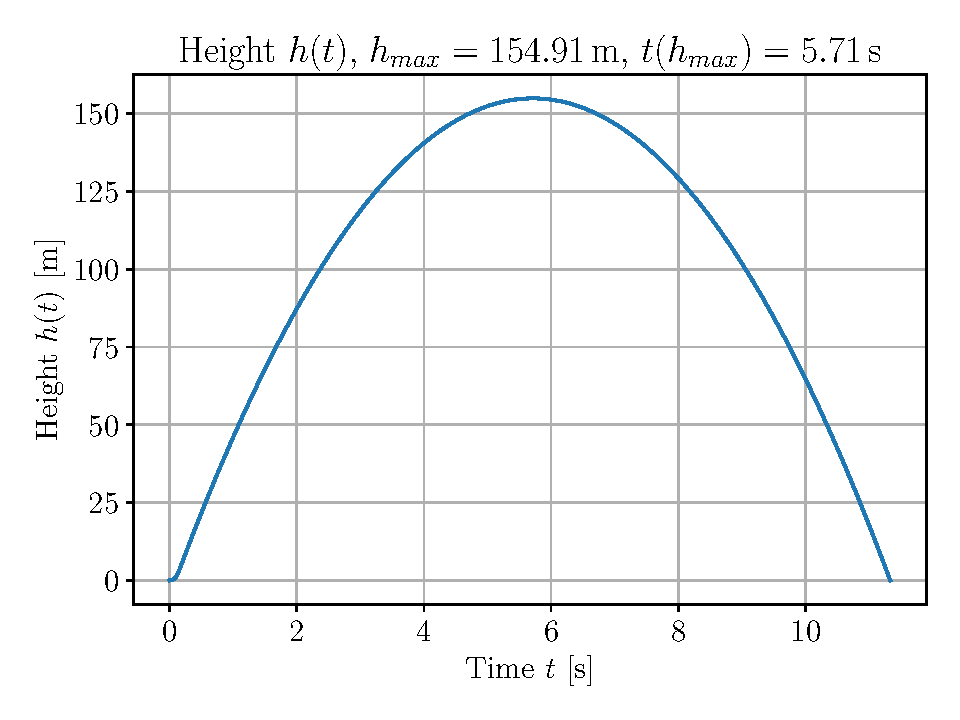
\includegraphics[width=\textwidth]{figures/h(t)_without_drag.pdf}
		\caption{Height $h(t)$ for a water rocket not experiencing drag forces.}
		\label{fig:h(t)_without_drag}
	\end{subfigure} \hfill
	\begin{subfigure}{0.49\textwidth}
		\centering
		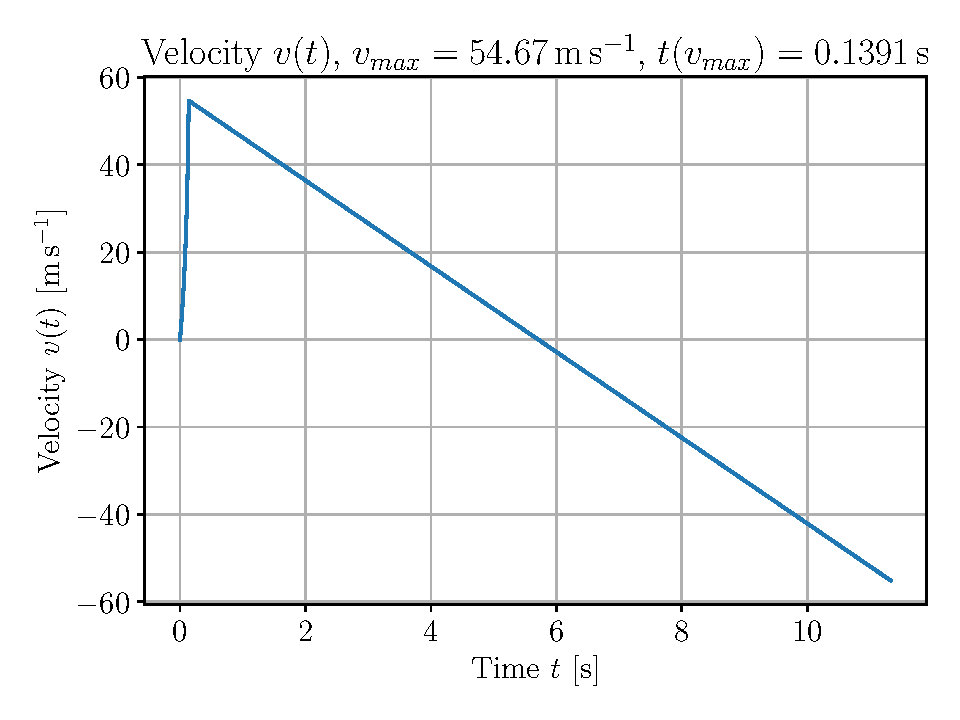
\includegraphics[width=\textwidth]{figures/v(t)_without_drag.pdf}
		\caption{Velocity $v(t)$ for a water rocket not experiencing drag forces.}
		\label{fig:v(t)_without_drag}
	\end{subfigure}
	\caption{Height and velocity profiles in dependence of time for a water rocket not experiencing drag forces.}
	\label{fig:results1_without_drag}
\end{figure}

As one can see from \cref{fig:h(t)_without_drag}, the maximal height achieved in the case of no drag forces acting upon the water rocket as it propagates through the air is roughly $\SI{155}{\meter}$ at time of roughly $\SI{6}{\second}$ after the start. Given real-life experiments using the mentioned parameters, one can interpret this result as not realistic, mainly because the water rocket is never observed to ascend to such heights as it would be predicted by a calculation without consideration of drag forces. The velocity curve $v(t)$ as shown \cref{fig:v(t)_without_drag} seems however to provide realistic estimates at least for the maximal velocity, which is around $\SI{55}{\meter\per\second}$ after approximately $\SI{140}{\milli\second}$ posterior to the start. Still, this would mean that the maximal velocity of the water rocket would be around $\SI{197}{\kilo\meter\per\hour}$; a velocity which water rockets in practical tests do not seem to achieve. It is however to be remembered, that the rocket does only travel at this maximal speed for a very short time, which could simply be too short to be observed consciously by eye of a human observer.

In conclusion nonetheless, the results for solving the rocket equation for a water rocket not experiencing drag forces seem to be exceedingly optimistic, such that they do not seem to give an appropriate description of the realistic behaviour of a water rocket in terms of achieved height $h(t)$ or velocity $v(t)$. The reason why drag forces are comparatively very important for water rockets is that their mass is very low compared to their size. A real rocket however has a lot more mass per cross-sectional area. For a water rocket therefore, it is paramount to solve the rocket equation under a proper consideration of drag forces.

\section{Solving the rocket equation for a water rocket with drag force}
It is not possible to solve the rocket equation analytically anymore, if drag forces are taken into consideration. In this section, the rocket equation with drag forces is therefore solved using the fourth-order Runge-Kutta method. Furthermore, example calculations are carried out and examined.

\subsection{Formulation of the rocket equation for a water rocket experiencing drag force}
In order to formulate the rocket equation for a rocket experiencing drag force, we start from \cref{eq:rocketeqsimple}. Now, in the case of non-negligible air resistance, the drag coefficient $\bar{C_{d}}$ is nonzero ans can be approximated by $\bar{C_{d}} = 0.57$ as given by \cref{eq:avdragvalue}; hence the second term in \cref{eq:rocketeqsimple} accounting for the drag force does not vanish. Therefore, the equation to proceed with is \begin{equation}
	m(t)\frac{\mathrm{d}v(t)}{\mathrm{d}t} = -\frac{\mathrm{d}m(t)}{\mathrm{d}t}v_p(t)\theta(\tau-t) - \frac{1}{2}\rho \bar{C}_d A v(t)^2 - m(t) g,
\end{equation} where $v_p(t) \geq 0$. Now, in our case we assume a constant propellant ejection velocity $v_p(t) = v_p$, whereas we further presuppose that the mass $m(t)$ is an affine function of time $t$, namely $m(t) = m_0 - bt$. Hereby, $b$ is the mass ejection parameter with units $[b] = \si{\kilogram\per\second}$ and $m_0$ is the mass of the rocket at time $t=0$. Inserting the expression for $m(t)$ into the above equation rearranging terms leads to the differential equation \begin{align}
\begin{aligned}\label{eq:rocketeqwithdragtointegrate}
\frac{\mathrm{d}v(t)}{\mathrm{d}t} = \frac{bv_p}{m_0-bt}\theta(\tau-t)-\frac{\gamma}{m_0-bt\theta(\tau-t)-b\tau\theta(t-\tau)}v(t)^2-g
\end{aligned},
\end{align} where $\gamma \doteq \tfrac{1}{2}\rho \bar{C_{d}} A$. With respect to time $t$, this equation can only be integrated using numerical methods, as compared to the rocket equation \cref{eq:rocketeqwithoutdragtointegrate} without drag forces there is now an additional term proportional to the square of the velocity $v(t)$ on the right hand side. We therefore need to resort to numerical methods to obtain solutions for the rocket equation taking drag forces into account.

\subsection{Numerical solution of the rocket equation for a rocket experiencing drag force}
In order to solve the rocket equation \cref{eq:rocketeqwithdragtointegrate} for a water rocket experiencing drag forces, we can use the fourth order Runge-Kutta scheme as derived in \cref{sec:derivrungekutta}. Using this method, one can solve for $v(t)$ and $h(t) = \frac{\mathrm{d}v(t)}{\mathrm{d}t}$ separately or simultaneously. In order to solve for both quantities simultaneously, two first-order differential equations have to be implemented in the algorithm, namely \begin{align}
	\begin{aligned}
		\frac{\mathrm{d}v(t)}{\mathrm{d}t} \doteq p(t, h(t), v(t))
	\end{aligned}
\end{align} and \begin{align}
\begin{aligned}
	\frac{\mathrm{d}h(t)}{\mathrm{d}t} \doteq f(t, h(t), v(t)).
\end{aligned}
\end{align} With regard to \cref{eq:rocketeqwithdragtointegrate}, the functions $p(t, h(t), v(t))$ and $f(t, h(t), v(t))$ are hereby defined as \begin{align}\footnotesize
\begin{aligned}\label{eq:reqdrag_rungekutta_1}
	p(t, h(t), v(t)) &= \frac{bv_p}{m_0-bt}\theta(\tau-t)-\frac{\gamma}{m_0-bt\theta(\tau-t)-b\tau\theta(t-\tau)}v(t)^2-g, \\
	f(t, h(t), v(t)) &= v(t).
\end{aligned}
\end{align} The time $t$ can be discretized to steps $t_i$ with $i \in \mathbb{N}_0$. Additionally, the notation $h(t_i) \doteq h_i$ and $v(t_i) \doteq v_i$ is adopted. The initial conditions for the integration problem are given by $t_0 = h_0 = v_0 = 0$. Now, let furthermore $\Delta t \in \mathbb{R}$ be the integration step-size giving the propagations $t_i \rightarrow t_{i+1} = t_i + \Delta t$, $h_i \rightarrow h_{i+1} = h(t_i+ \Delta t)$ and $v_i \rightarrow v_{i+1} = v(t_i + \Delta t)$.

The fourth-order Runge-Kutta scheme now gives the iterations $t_i \rightarrow t_{i+1}$, $h_i \rightarrow h_{i+1}$ and $v_i \rightarrow v_{i+1}$ as \begin{align}
	\begin{aligned}\label{eq:reqdrag_rungekutta_2}
		t_{i+1} &= t_i + \Delta t, \\
		h_{i+1} &= h_i + \frac{\Delta t}{6}(k_1^h+2k_2^h+2k_3^h+k_4^h), \\
		v_{i+1} &= v_i + \frac{\Delta t}{6}(k_1^v+2k_2^v+2k_3^v+k_4^v),
	\end{aligned}
\end{align} where the quantities $k_\mu^\nu$ with $\mu \in \{1,2,3,4\}$ and $\nu \in \{h,v\}$ are calculated as \begin{align}
\begin{aligned}\label{eq:reqdrag_rungekutta_3}
	k_1^h &= f(t_i,h_i,v_i), \\
	k_1^v &= p(t_i,h_i,v_i), \\
	k_2^h &= f\left(t_i+\frac{\Delta t}{2}, h_i + \frac{\Delta t}{2}k_1^h, v_i + \frac{\Delta t}{2}k_1^v\right), \\
	k_2^v &= p\left(t_i+\frac{\Delta t}{2}, h_i + \frac{\Delta t}{2}k_1^h, v_i + \frac{\Delta t}{2}k_1^v\right), \\
	k_3^h &= f\left(t_i+\frac{\Delta t}{2}, h_i + \frac{\Delta t}{2}k_2^h, v_i + \frac{\Delta t}{2}k_2^v\right), \\
	k_3^v &= p\left(t_i+\frac{\Delta t}{2}, h_i + \frac{\Delta t}{2}k_2^h, v_i + \frac{\Delta t}{2}k_2^v\right), \\
	k_4^h &= f\left(t_i+\Delta t, h_i + \Delta tk_3^h, v_i + \Delta t k_3^v\right), \\
	k_4^v &= p\left(t_i+\Delta t, h_i + \Delta tk_3^h, v_i + \Delta t k_3^v\right).
\end{aligned}
\end{align} The three expressions \cref{eq:reqdrag_rungekutta_1}, \cref{eq:reqdrag_rungekutta_2} and \cref{eq:reqdrag_rungekutta_3} hence define the equations to implement in an algorithm intended to solve the rocket equation \cref{eq:rocketeqwithdragtointegrate} with drag forces for the velocity $v(t)$ and the height $h(t)$ in a desired time window.

\subsection{Actual calculations and results}
In order to do actual calculations for the rocket velocity $v(t)$ and the rocket height $h(t)$ in the case of a rocket experiencing drag forces, the propellant ejection time $\tau$, the propellant ejection  velocity $v_p$ and the mass ejection parameter $b$ have to be known as in the case of a rocket with negligible drag forces acting upon it. Given the assumptions, that the propellant ejection be constant over the whole period of ejection and that furthermore the pressure inside the tank ejecting the propellant can be approximated by the average pressure over the ejection time, these quantities can be calculated by \cref{eq:propellantejectiontime}, \cref{eq:propellantejectionvelocity} and \cref{eq:freeparameters}. The results as shown in this subsection were obtained\footnote{The code which produces the results as shown here is found at \url{https://github.com/danielzahnd/water-rocket/blob/main/code/water_rocket_air_resistance.ipynb}.} for a pressure $P_0 = \SI{8}{\bar}$, a typical half-liter PET plastic bottle of mass $m_r \approx \SI{40}{\gram}$, an exhaust radius of $r = \SI{4.5}{\milli\meter}$ and a propellant mass of $m_w = \SI{0.25}{\kilo\gram}$. The cross-sectional radius of the plastic bottle is $R \approx \SI{3.25}{\centi\meter}$.
\begin{figure}[h]
	\begin{subfigure}{0.49\textwidth}
		\centering
		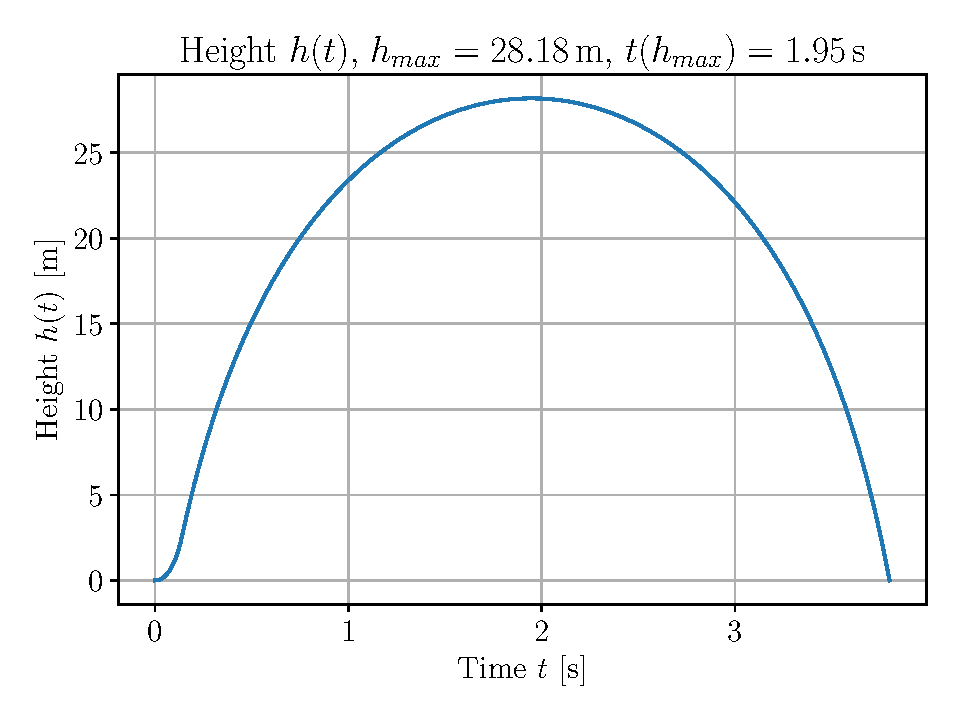
\includegraphics[width=\textwidth]{figures/h(t)_with_drag.pdf}
		\caption{Height $h(t)$ for a water rocket experiencing drag forces.}
		\label{fig:h(t)_with_drag}
	\end{subfigure} \hfill
	\begin{subfigure}{0.49\textwidth}
		\centering
		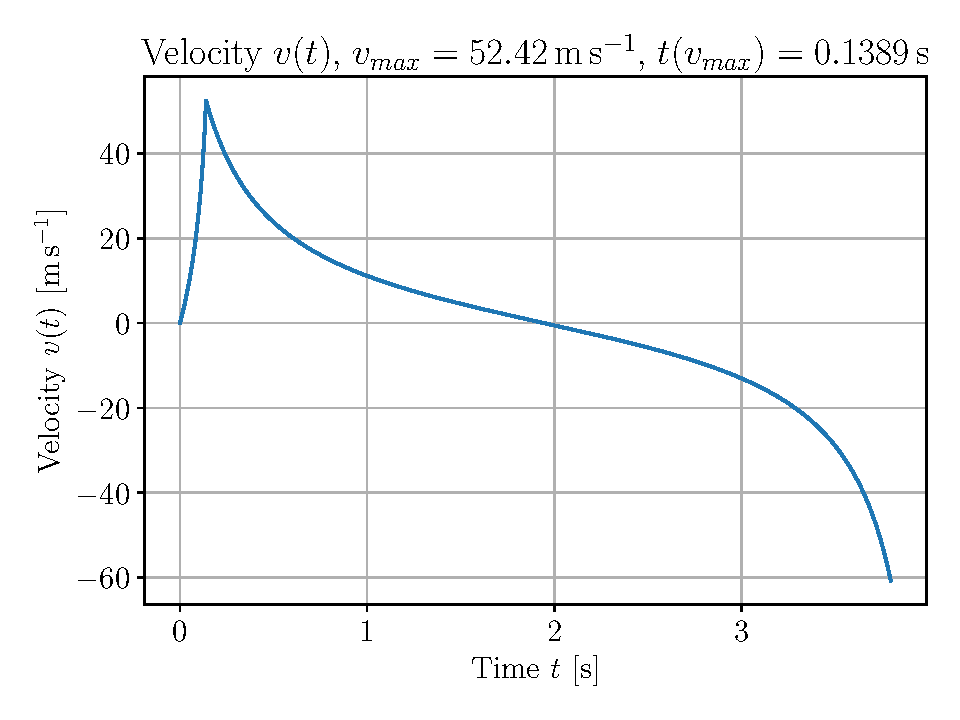
\includegraphics[width=\textwidth]{figures/v(t)_with_drag.pdf}
		\caption{Velocity $v(t)$ for a water rocket experiencing drag forces.}
		\label{fig:v(t)_with_drag}
	\end{subfigure}
	\caption{Height and velocity profiles in dependence of time for a water rocket experiencing drag forces.}
	\label{fig:results1_with_drag}
\end{figure}

First of all, the acceleration phase as seen in \cref{fig:v(t)_with_drag} seems to be almost equal to the case without drag forces, as the $t(v_{max})$ values for both cases are roughly equal to one another. Also the values for the maximal velocities are similar for both cases. However, the case taking into account drag forces renders the more realistic value of roughly $v_{max} \approx \SI{52}{\meter\per\second} \approx \SI{189}{\meter\per\second}$. In practical experiments however, this velocity still does not seem to be achieved. But one has to note here, that the phase during which the water rockets would travel at that velocity is very short, such that it is likely almost unperceivable by the human eye.

As for the height results, we seem to obtain realistic results. The total time for the rocket to reach maximal height with roughly two seconds seems to correspond well to practical experiments, at least a lot better than the value of roughly six seconds as for the case without drag forces. Also the predicted maximal height of roughly 28 meters is very realistic, given observations in field experiments. This is not really surprising, since it was already established that a consideration of drag forces is paramount to calculations for a water rocket. An explanation for this is found by examining \cref{eq:rocketeqwithdragtointegrate}. Hereby, the term accounting for drag forces is proportional to the ratio $A/m(t)$. Hence, if this ratio is large, drag forces are dominant, whereas they are negligible if $A/m(t) \ll 1$. For real rockets, the $A/m(t) \ll 1$ holds, whereas for water rockets it is given\footnote{Hereby, the values $m_r \approx \SI{0.04}{\kilogram}$ and $A = R^2\pi$ with $R \approx \SI{3.25}{\centi\meter}$ were used for an estimation of the cross-sectional area to mass ratio.} by $A/m_r \approx \SI{0.08}{\meter^2\kilogram^{-1}}$. A corresponding calculation for the unfuelled starship rocket of SpaceX yields $A/m_r \approx \SI{0.0002}{\meter^2/\kilogram^{-1}}$ and is therefore roughly 400 times smaller than for the water rocket. This is why drag forces are largely negligible in the latter case, but not for water rockets due to their large cross-sectional area to mass ratio.

In conclusion, the calculations as found in this section considering drag forces seem to give realistic estim
ates for the real-world case as observed in field experiments. Using the code and the equations, one can experiment with different propellant masses $m_w$ and start pressure values $P_0$ needed to obtain maximal height.

\appendix
\chapter{Derivation of the Bernoulli equation}
Consider a fluid flowing in a pipe as shown in \cref{fig:bernoulliderivation}; furthermore let $\Delta V$ with mass $\Delta m = \rho\Delta V$ denote a small fluid portion moving along a streamline from the right to the left, where $\rho$ is the constant fluid density. The total work done on/by the fluid portion  $W_{tot}$ is given by \begin{equation}
W_{tot} = \Delta E_{kin} + \Delta E_{pot}.
\end{equation}
\begin{figure}[h]
\centering
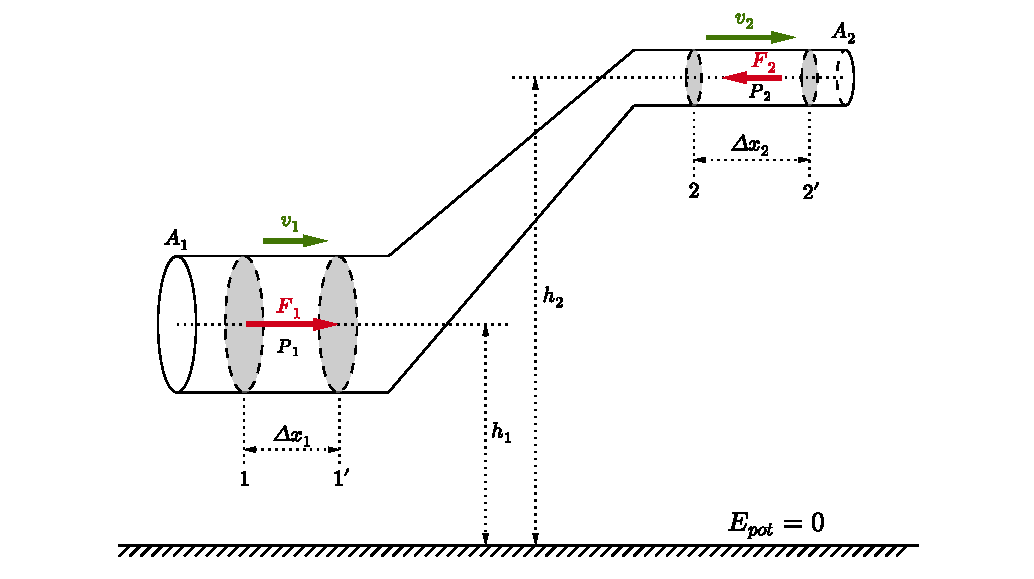
\includegraphics[width=12cm]{figures/bernoulliderivation.pdf}
\caption{Sketch for the derivation of the Bernoulli equation.}
\label{fig:bernoulliderivation}
\end{figure} Due to the conservation of energy, the change in potential energy $\Delta E_{pot}$ can be calculated by \begin{equation}
\Delta E_{pot} = \Delta m g h_2 - \Delta m g h_1 = \rho \Delta V g (h_2-h_1).
\end{equation} The change in kinetic energy $\Delta E_{kin}$ however can be written as \begin{equation}
\Delta E_{kin} = \frac{1}{2}\Delta m \vect{v}_2^2 - \frac{1}{2}\Delta m \vect{v}_1^2 = \frac{1}{2}\rho \Delta V (\vect{v}_2^2-\vect{v}_1^2).
\end{equation} The force $\vect{F}_1$ pushing the fluid element from $1$ to $1^\prime$ can be written by  $\vect{F}_1 = A_1P_1\vect{e}_x$; furthermore the force $\vect{F}_2$ opposing the fluid movement from $2$ to $2^\prime$ is given by $\vect{F}_2 = -A_2 P_2\vect{e}_x$. The work $W_1$ done for the fluid movement $1\rightarrow 1^\prime$ is calculated as $W_1 = |\vect{F}_1|\Delta x_1 = P_1A_1\Delta x_1 = P_1\Delta V$, whereas the work $W_2$ done for the fluid movement $2\rightarrow 2^\prime$ is given by $W_2 = -|\vect{F}_2|\Delta x_2 = -P_2A_2\Delta x_2 = -P_2\Delta V$. The total work $W_{tot}$ can then be written by means of the equation \begin{gather}
W_{tot} = W_1 + W_2 = \Delta E_{kin} + \Delta E_{pot} = (P_1-P_2)\Delta V.
\end{gather} Plugging in the expressions for $\Delta E_{pot}$ and $\Delta E_{kin}$, the equation \begin{equation}
\rho \Delta V g (h_2-h_1) + \frac{1}{2}\rho \Delta V (\vect{v}_2^2 - \vect{v}_1^2) = (P_1-P_2)\Delta V
\end{equation} results. After rearranging terms and dividing by $\Delta V$, the Bernoulli equation \begin{equation}
P_1 + \rho g h_1 + \frac{1}{2}\rho \vect{v}_1^2 = P_2 + \rho g h_2 + \frac{1}{2}\rho \vect{v}_2^2
\end{equation} obtains. Assuming, that this equation reflects a stationary state at a fixed time $t$ and further assuming that $P_1 = P(\vect{x}_1,t)$, $P_2 = P(\vect{x}_2,t)$, $h_1 = h(\vect{x}_1,t)$, $h_2 = h(\vect{x}_2,t)$, $\vect{v}_1 = \vect{v}(\vect{x}_1,t)$ and $\vect{v}_2 = \vect{v}(\vect{x}_2,t)$, the Bernoulli equation can also be written in the form \begin{equation}
P(\vect{x},t)| + \rho g h(\vect{x},t)+ \frac{1}{2}\rho \vect{v}(\vect{x},t)^2 = \text{const.}
\end{equation} indicating, that pressure, velocity and height of a fluid element sum to a constant value in the specified combination at all times and places along a streamline.

\chapter{Derivation of the drag equation}
Consider a fluid of constant density $\rho$ flowing horizontally around a massive object, as seen in \cref{fig:dragequationderivation}.
\begin{figure}[h]
\centering
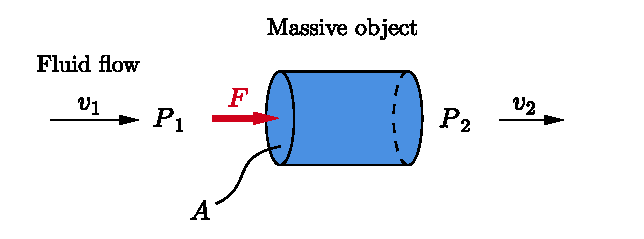
\includegraphics[width=9cm]{figures/dragequationderivation.pdf}
\caption{Sketch for the derivation of the drag equation.}
\label{fig:dragequationderivation}
\end{figure}
Assuming, that the fluid velocity $|\vect{v}_2|$ behind the object is zero and that the fluid does not undergo any height change with respect to some reference height, the Bernoulli equation yields \begin{equation}
P_1 + \frac{1}{2}\rho \vect{v}_1^2 = P_2 \quad \Leftrightarrow \quad \Delta P \doteq P_2-P_1 = \frac{1}{2}\rho \vect{v}_1^2.
\end{equation} A change of pressure $\Delta P$ in the fluid going from the front of the object to the back of it implies, that there is a force $F \doteq |\vect{F}|$ exerted by the fluid on the object. Writing $\vect{v} \doteq \vect{v}_1$, the magnitude of $F$ is given by the equation \begin{equation}
F = A \Delta P = \frac{1}{2}\rho A \vect{v}^2.
\end{equation} In general, the fluid velocity is dependent upon time, therefore $\vect{v} = \vect{v}(t)$; furthermore, the density of the fluid can be spatially variable, hence $\rho = \rho(\vect{x})$. Now, if an object of arbitrary shape moving with the velocity $\vect{v}(t)$ within a stationary fluid is considered, the drag force $\vect{F}_d(\vect{x},t)$ it experiences is directly opposing the direction of movement and can be written by \begin{equation}
\vect{F}_d(\vect{x},t) = - \frac{1}{2}\rho(\vect{x})C_d A \frac{\vect{v}(t)^3}{|\vect{v}(t)|},
\end{equation} where $C_d$ is a scaling factor to be experimentally determined related to the geometry of the object under consideration. Drag coefficients for different object geometries can be taken from \cref{fig:dragcoefficients}.

\chapter{Derivation of the rocket equation}
Consider a situation, where one has rocket of mass $m(t)$ ascending in positive vertical direction $\vect{e}_z$, where the speed of the rocket is denoted by $\vect{v}(t)$ and the propellant is ejected with velocity $\vect{v}_p(t)$ in negative vertical direction, that is $-\vect{e}_z$. This situation is shown in \cref{fig:rocketequation}, where $\vect{F}_p$ denotes the force generated by the propellant ejection, $\vect{F}_g$ is the force due to gravity, $\vect{F}_d$ is the drag force the rocket experiences and $\vect{F}$ is the net force acting upon the rocket. 
\begin{figure}[h]
	\centering
	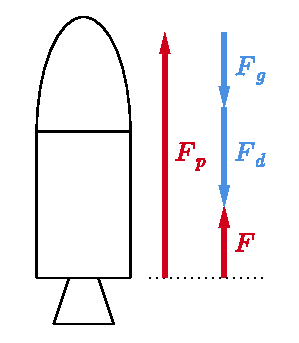
\includegraphics[width=4cm]{figures/rocketequationderivation.pdf}
	\caption{Sketch for the derivation of the general rocket equation considering drag force $\vect{F}_d$, gravitational force $\vect{F}_g$, propellant force $\vect{F}_p$ and a net force $\vect{F}$.}
	\label{fig:rocketequation}
\end{figure} In general, all of these forces are time-dependent. First of all, the force due to the propellant ejection can be accounted for by \begin{equation}
\vect{F}_p(t) = \vect{v}_p(t)\frac{\mathrm{d}m(t)}{\mathrm{d}t}\theta(\tau-t),
\end{equation} where $\theta: \mathbb{R}\rightarrow \{0,1\}$ is the Heaviside function, $\tau$ is the total time of propellant ejection and $\vect{v}_p(t)$ is the in general time-dependent ejection velocity of the propellant, which is oriented towards the negative vertical axis; that is to say, against the movement direction of the rocket. Furthermore, the force due to gravity is given as \begin{equation}
\vect{F}_g(t) = -m(t)g\vect{e}_z,
\end{equation} where $m(t)$ is the time-dependent mass of the rocket and $g=\SI{9.81}{\meter\second^{-2}}$ is the gravitational acceleration assumed as constant for all reached heights of the rocket. Lastly, the force due to air resistance (drag) is accounted for by the drag equation as \begin{equation}
\vect{F}_d(t) = -\frac{1}{2}\rho(\vect{x})\vect{v}(t)^2 \bar{C}_d A \vect{e}_z,
\end{equation} where $\rho(\vect{x})$ is the air density at $\vect{x}$, $\bar{C}_d$ is the drag coefficient of the rocket and $A$ is the cross-sectional area of the rocket with respect to its propagation direction.

From \cref{fig:rocketequation} it can be derived, that the net force $\vect{F}(t)$ is given by the sum \begin{equation}\label{eq:sumforces}
\vect{F}(t) = \vect{F}_p(t) + \vect{F}_d(t) + \vect{F}_g(t).
\end{equation} According to Newton's second law, this net force can be written as \begin{equation}
\vect{F}(t) = m(t)\frac{\mathrm{d}\vect{v}(t)}{\mathrm{d}t},
\end{equation} thus leading to the full rocket equation accounting for air resistance obtained by inserting the above expressions for each force into \cref{eq:sumforces}, namely \begin{equation}
m(t)\frac{\mathrm{d}\vect{v}(t)}{\mathrm{d}t} = \frac{\mathrm{d}m(t)}{\mathrm{d}t}\vect{v}_p(t)\theta(\tau-t) - \frac{1}{2}\rho(\vect{x})\vect{v}(t)^2\bar{C}_dA\vect{e}_z - m(t)g\vect{e}_z.
\end{equation}

\chapter{Derivation of the Runge-Kutta scheme}\label{sec:derivrungekutta}
The derivation of the fourth-order Runge-Kutta integration scheme is a lengthy task, which is in principle not complicated, but tedious; therefore only the key steps are outlined here.

The fourth-order Runge-Kutta scheme solves a differential equation of the form \begin{equation}
\frac{\mathrm{d}\vect{y}(t)}{\mathrm{d}t} = \vect{f}(t,\vect{y})
\end{equation} numerically. The fourth-order refers to the number of vectors $\vect{k}_i,\,i\in\mathbb{N}$ used in order to propagate the solution $\vect{y}(t)$ from a state $t$ to a state $t+\Delta t$ with $\Delta t\in\mathbb{R}$; in the fourth-order case four vectors $\vect{k}_i,\,i\in\{1,\dots,4\}$ are thus needed. The fourth-order Runge-Kutta scheme is given by \begin{align}
\begin{aligned}
\vect{k}_1 &= \vect{f}(t_k,\vect{y}_k) \\
\vect{k}_2 &= \vect{f}(t_k+\nicefrac{1}{2}\Delta t,\vect{y}_k+\nicefrac{1}{2}\vect{k}_1) \\
\vect{k}_3 &= \vect{f}(t_k + \nicefrac{1}{2}\Delta t,\vect{y}_k+\nicefrac{1}{2}\vect{k}_2) \\
\vect{k}_4 &= \vect{f}(t_k+\Delta t,\vect{y}_k+\vect{k}_3) \\
\vect{y}_{k+1} &= \vect{y}(t_{k+1}) = \vect{y}_k + \frac{\Delta t}{6}\left(\vect{k}_1 + 2\vect{k}_2 + 2\vect{k}_3 + \vect{k}_4\right),
\end{aligned}
\end{align}
where $\Delta t\in\mathbb{R}$ is the step-size parameter. In \cref{fig:rungekutta}, a sketch of the functionality for the Runge-Kutta scheme can be seen.

\begin{figure}[h]
\centering
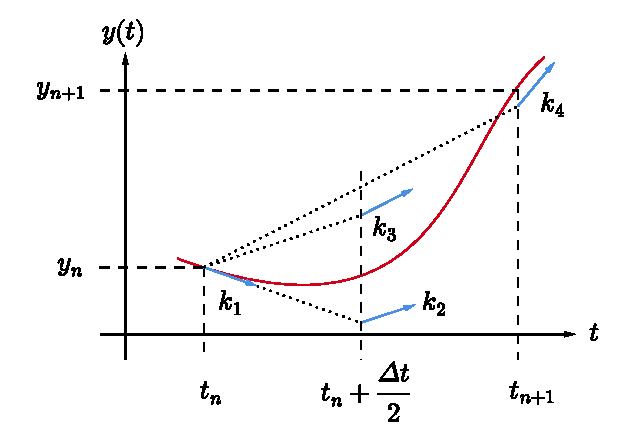
\includegraphics[width=9cm]{figures/rungekutta.pdf}
\caption{Sketch of the functionality for the fourth-order Runge-Kutta scheme. The shown coordinate system is to be understood as simplified representation of the $n$-dimensional vector $\vect{y}(t)$ in a two-dimensional coordinate system.}
\label{fig:rungekutta}
\end{figure}

In order to derive this result, the ansatz
\begin{align}\small
\begin{aligned}
\vect{k}_1 &= \vect{f}(t_k,\vect{y}_k) \\
\vect{k}_2 &= \vect{f}(t_k+\alpha_{2,1}\Delta t,\vect{y}_k+\alpha_{2,1}\vect{k}_1) \\
\vect{k}_3 &= \vect{f}(t_k + \alpha_{3,1}\Delta t + \alpha_{3,2}\Delta t,\vect{y}_k+\alpha_{3,1}\vect{k}_1 + \alpha_{3,2}\vect{k}_2) \\
\vect{k}_4 &= \vect{f}(t_k+\alpha_{4,1}\Delta t + \alpha_{4,2}\Delta t + \alpha_{4,3}\Delta t,\vect{y}_k+\alpha_{4,1}\vect{k}_1 + \alpha_{4,2}\vect{k}_2 + \alpha_{4,3}\vect{k}_3) \\
\vect{y}_{k+1} &= \vect{y}(t_{k+1}) = \vect{y}_k + \Delta t \left(\beta_1 \vect{k}_1 + \beta_2\vect{k}_2 + \beta_3\vect{k}_3 + \beta_4\vect{k}_4\right),
\end{aligned}
\end{align}
is made inspired by visual considerations as seen in \cref{fig:rungekutta}. Next, optimal values for the parameters in the set \begin{equation} C \doteq \{\alpha_{2,i}, \alpha_{3,j}, \alpha_{4,k}, \beta_l\}, \, i \in \{1\},\,j \in \{1,2\},\,k \in \{1,2,3\},\, l \in \{1,2,3,4\}
\end{equation} are desired to be found; to this end, the following steps are carried out as outlined:
\begin{enumerate}
\item Expand $\vect{y}_{k+1}$ with $t_{k+1} = t_k +\Delta t$ into a third-order Taylor expansion around $t_k$, neglecting terms of order $\mathcal{O}(\Delta t^5)$.
\item Expand expressions for $\vect{k}_1$, $\vect{k}_2$, $\vect{k}_3$ and $\vect{k}_4$ around $\Delta t=0$ up to fourth order, neglecting terms of order $\mathcal{O}(\Delta t^5)$.
\item Calculate $\vect{y}_{k+1} = \vect{y}_k + \Delta t(\beta_1\vect{k}_1 + \beta_2\vect{k}_2 + \beta_3\vect{k}_3 + \beta_4\vect{k}_4)$ with the expanded $\vect{k}_i$-vectors for $i \in \{1,\dots,4\}$.
\item Force this expression to resemble the Taylor expansion from step 1 by equating expressions of same order in $\Delta t$.
\item Get conditional equations for coefficient set $C$.
\end{enumerate}
Using this procedure, one ends up with the fourth-order Runge-Kutta scheme as stated above.

%\chapter{How to build a water rocket}
%Text.

%\bibliography{references}
%\bibliographystyle{apalike}

\end{document}